\documentclass{beamer}
%% Possible paper sizes: a0, a0b, a1, a2, a3, a4.
%% Possible orientations: portrait, landscape
%% Font sizes can be changed using the scale option.
\usepackage[size=a3,orientation=landscape,scale=1.8]{beamerposter}
\usetheme{LLT-poster}
% \usecolortheme{ComingClean}
\usecolortheme{Entrepreneur}
% \usecolortheme{ConspiciousCreep}  %% VERY garish.

\usepackage[utf8]{inputenc}
\usepackage[T1]{fontenc}
\usepackage{libertine}
\usepackage[scaled=0.92]{inconsolata}
\usepackage[libertine]{newtxmath}

\usepackage{mwe}
\author[Ruibo Gai]{Group 15:}
\title{Discussing Six Thinking Hats:\\ Creative Decision-Making}
\footimage{
\includegraphics[width=4cm]{Durham Logo.png}}
\institute{Tianchen Yan}
\definecolor{mycolor}{RGB}{93, 144, 192}
\begin{document}
\begin{frame}[fragile]
\begin{columns}[T]

%%%% First Column
\begin{column}{.33\textwidth}
\begin{block}{Purposes of this method}
\begin{itemize}
\item The Six Thinking Hats method serves several purposes and holds significant value in various contexts. 
\item It is a valuable tool for structured thinking, creativity, and decision-making, offering numerous benefits in terms of problem-solving effectiveness, innovation, communication, and collaboration.
\item Its systematic approach and versatility make it a widely used and highly regarded technique in various professional and personal settings.
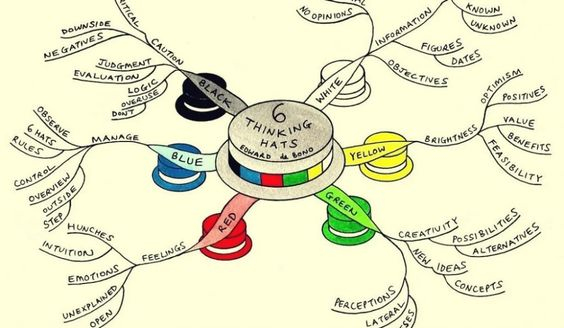
\includegraphics[width=.8\linewidth]{branches.jpg}
\end{itemize}
\end{block}


\begin{block}{Benefits of this method}
\begin{itemize}
\item A meeting facilitation tool that surfaces hidden agendas and achieves objectives without conflict.
\item A way to make sure that all sides of an issue are addressed.
\item A tool that works well in different cultures around the world.
\item A sharpened ability to think clearly, objectively, systematically, and creatively.
\end{itemize}
\end{block}
\end{column}

%%Second column
\begin{column}{.33\textwidth}
\begin{block}{Overview}
\begin{itemize}
\item \textcolor{mycolor}{What is six thinking hats?}\\
The Six Thinking Hats, a strategy devised by Edward de Bono, is a dynamic approach to exploring different perspectives in decision-making. Each hat represents a distinct mode of thinking. 
\end{itemize}
\begin{center}
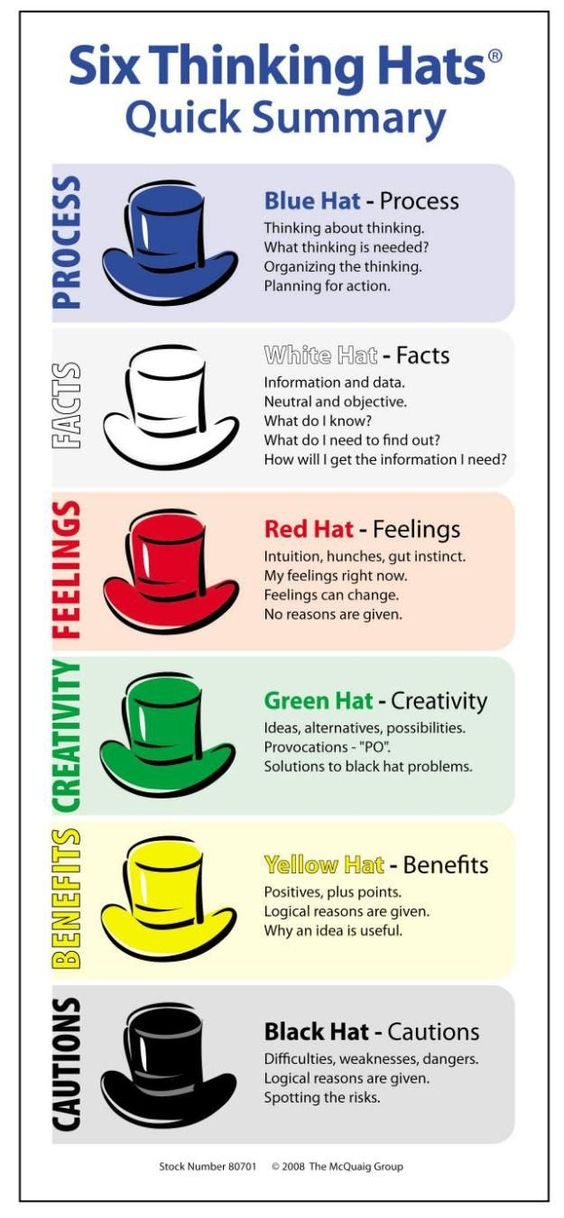
\includegraphics[width=.6\linewidth]{What.jpg}
\end{center}
\end{block}
\end{column}


%%%% Third Column
\begin{column}{.3\textwidth}


\begin{block}{Tips for Implementation}
\begin{itemize}
\item \textcolor{mycolor}{Set Clear Objectives:} \\
\hspace*{1em}Define the purpose and goals of the session.Clearly communicate what you aim to achieve with the Six Thinking Hats method, whether it's brainstorming new ideas, solving a specific problem, or making a decision.

\item \textcolor{mycolor}{Use Visual Aids:}\\
  \hspace*{1em}Utilize visual aids, such as diagrams or slides, to reinforce key concepts and keep participants engaged. Visual representations of the hats and their respective roles can help clarify the method and guide discussions.
\item \textcolor{mycolor}{Rotate Hats Regularly:} \\
  \hspace*{1em} Encourage participants to switch between hats regularly throughout the session. Set specific time intervals for each hat or transition to a new hat when the discussion reaches a natural break point.
\item \textcolor{mycolor}{Facilitate Open Communication:} \\
  \hspace*{1em}Promote open dialogue for all to share ideas freely. Value every suggestion to spark creativity and enhance team collaboration and respect.
\end{itemize}


\includegraphics[width=.6\linewidth]{let_s_learn.png}
\end{block}
\end{column}


\end{columns}

%%%% This is the THIRD column



\end{frame}
\end{document}